\documentclass[12pt, twoside]{article}

\usepackage{amsfonts}
%\usepackage[T1]{fontenc}
%\usepackage[ansinew]{inputenc}
\usepackage{amssymb}
\usepackage{amsthm}
\usepackage{amsmath}
% \usepackage{ mathrsfs }
\usepackage{dsfont}
\usepackage{natbib}
\setlength{\bibsep}{0pt plus 100ex}
\usepackage{url}
\usepackage{pdflscape}
\usepackage{pdfpages}
\usepackage{svg}
\usepackage[utf8]{inputenc}
\usepackage{graphicx}
\usepackage{bbold}


\usepackage{enumitem}
%\usepackage[german,  onelanguage, linesnumbered]{algorithm2e}
\usepackage{placeins}
\usepackage{a4}
\usepackage[a4paper, ]{geometry}
\geometry{
 a4paper,
 right=30mm,
 left=30mm,
 top=30mm,
 }

% For tables
\usepackage{tabularx}
\usepackage{multirow}
\usepackage{pbox}

% \usepackage{color}

\widowpenalty = 5000
\clubpenalty = 5000


\newcommand{\Prob}{\mathbb{P}}
\newcommand{\V}{\mathbb{V}}
\newcommand{\Cov}{\text{Cov}}
\newcommand{\E}{\mathbb{E}}
\newcommand{\R}{\mathbb{R}}
\newcommand{\N}{\mathbb{N}}
\newcommand{\1}{\mathbb{1}}
\newcommand{\LL}{\mathcal{L}}
\newcommand{\F}{\mathcal{F}}
\newcommand{\iid}{\overset{\text{iid}}{\sim}}
\newcommand{\SUM}{\sum_{i=1}^n}
\newcommand{\PROD}{\prod_{i=1}^n}



\begin{document}

\begin{titlepage}

    \newcommand{\HRule}{\rule{\linewidth}{0.5mm}} % Defines a new command for the horizontal lines, change thickness here

    \center % Center everything on the page
 
    %----------------------------------------------------------------------------------------
    %	HEADING SECTIONS
    %----------------------------------------------------------------------------------------
    
\includegraphics[scale = 0.22]{campus-seal.jpg}\\[0.5cm]
    
     \textsc{\large University of California, Los Angeles}\\[0.2cm] % Minor heading such as course title
     \textsc{\large Department of Statistics}\\[0.5cm]
    %----------------------------------------------------------------------------------------
    %	TITLE SECTION
    %----------------------------------------------------------------------------------------

    \HRule \\[0.4cm]
    { \huge \bfseries Imputation of Missing Values in CART}\\[0.2cm] % Title of your document
    \HRule \\[0.4cm]
    \textsc{\large An Application of the EM Algorithm
    }\\[2.0 cm]
 
    %----------------------------------------------------------------------------------------
    %	AUTHOR SECTION
    %----------------------------------------------------------------------------------------
    
    \hspace{1cm}
    \begin{minipage}{0.4\textwidth}
    \begin{flushleft} \large
    \emph{Author:}\\
        Thomas \textsc{Maierhofer}\\
        SID 905078249 % Your name
    \end{flushleft}
    \end{minipage}
    ~
    \begin{minipage}{0.4\textwidth}
    \begin{flushright} \large
    \emph{Stats 201C:} \\
    Prof. Quing Zhou \\ % Supervisor's Name
    \text{}
    \end{flushright}
    \end{minipage}\\[1.5cm]
    
    \large{
    Final Project Report
    } \\[1.5cm]
    
    {\large Spring Quarter 2019,} \\
    {\large June 14, 2019}\\[2cm] % Date, change the \today to a set date if you want to be precise

    %----------------------------------------------------------------------------------------

    \vfill % Fill the rest of the page with whitespace

\end{titlepage}

%\newpage
%\hspace{5cm}
%\newpage

\pagenumbering{roman}
\tableofcontents 
\clearpage

\begin{abstract}
Classification and Regression Trees (CART) are one of the most widely used algorithms in machine learning. 
There are multiple ways of treating missing values in covariates, many of which work well in different scenarios. This report proposes a novel strategy for imputing missing values based on an EM algorithm. In the expectation step (E step), missing values are imputed based on the leaf node in which they fall given the current CART. In the maximization step (M step), the CART is fit on the current training data. These steps are repeated until convergence, i.e.\ the imputed values do not change anymore. 
Using a simulation study, this EM algorithm is shown to achieve superior predictive performance in comparison with a number of traditional treatments of missing values in CART.


\end{abstract}
\clearpage
\pagenumbering{arabic}

\section{Background}
This section introduces the two cornerstones of this report: Classification and Regression Trees (CART) in Section~\ref{CART} and the EM algorithm in Section~\ref{EM_algorithm}. 

\subsection{Classification And Regression Trees}\label{CART}
Classification and Regression Trees (CART) were originally introduced by \cite{breiman1984} and have quickly gained popularity due to their competitive predictive power, simple implementation, and easily comprehensible concept.
CARTs create a model based on a recursive algorithm that splits the covariate space into more homogeneous (w.r.t. the target variable) subspaces, a.k.a.\ nodes, using binary splits on individual covariates. The final nodes are called leaves and are used for prediction.
The algorithm for CART works as follows:

\fbox{ \centering{
\parbox{0.9\textwidth}{\textbf{Creating CART}
\begin{enumerate}
    \item Initialize the empty tree with the root node containing all observations
    \item For each node not satisfying the stopping criterion: \label{step:CART_split}
    \begin{enumerate}[label*=\arabic*]
        \item Find the split that minimizes the node impurity in its resulting child nodes
        \item Add child nodes to the tree.
    \end{enumerate}
    \item While stopping criteria of the tree are not reached repeat Step~\ref{step:CART_split}
    \item Return tree with splits and nodes
\end{enumerate}
}}}

Note that all splits are binary splits on one of the covariates. Common stopping criteria for nodes are its minimal nodesize or minimal impurity. Nodes that are not split any further are called leaf nodes.
A common stopping criteria for the overall tree is its depth, i.e.\ maximal number of recursive splits. 
Most commonly, a CART is depicted in a tree structure, see Figure~TODO, but for two dimensional carts the splits can be shown in a planar colormap, see Figure~TODO.


\subsection{Expectation Maximization Algorithm}\label{EM_algorithm}
The EM algorithm is an iterative algorithm for obtaining the maximum likelihood estimator for parameters in a statistical model under the presence of unobserved variables. 
The basic concept of the EM algorithm has been used for a long time but was explicitly formalized by \cite{dempster1977maximum}.
It iterates between the expectation step (E step), where the parameters of the model are used to obtain the (expectation of) the unobserved variables, and the maximization step (M step), where the model parameters are chosen to maximize the likelihood given the estimated (originally unobserved, now observed) variables.

\section{Treatment of Missing Values in CART}\ref{treatment_of_missing_values_in_cart}
This section introduces an EM algorithm for the treatment of missing values in CARTs in Section~\ref{EM_for_CART} after a brief review of commonly used methods in Section~\ref{traditional_methods}.

\subsection{Traditional Methods}\label{traditional_methods}
The most obvious way of treating missing values in a CART (and any other statistical model) is to simply delete observations with missing values. This is problematic if the data is not missing completely at random (MCAR) or if there are not enough complete pbservatiosn left to fit a reasonable model. 
Alternatively, missing values can be imputed using arithmetic means for scalar variables and modes for categorical variables. This ad-hoc method generally provides good results for MCAR data.
Both approaches are very problematic if the data is jsut missing at random (MAR) conditional on the observed data. This is a cmmon assumption, mainly because without it asymptotically true estimators cannot be obtained.

\subsection{EM Algorithm}\label{EM_for_CART}
The EM algorithm for the treatment of missing values in CARTs finds the maximum likelihood estimator for the model given its unobserved observations. It has the advantage, that asymptotically it will recover the true model parameters even if the missing values are MAR, i.e. they depend on the observed data.
In its E step, missing values are imputed based on the leaf node in which the observations falls given the current CART. Missing values in scalar covariates are imputed as the arithmetic mean of all observations within the leaf node, categorical covariates as the majority class (mode).
In its M step, the CART is fit on the current data. 
These steps are repeated until convergence, i.e.\ the imputed values do not change anymore. 
In pseudocode, this algorithm is:

\fbox{ \centering{
\parbox{0.9\textwidth}{\textbf{EM for Missing Values in CART}
\begin{enumerate}
    \item Initialize missing values as random draws from their (observed) marginal distribution
    \item Fit initial CART on completed data
    \item \textbf{E step}: Impute missing values based on current model \label{step:E_step}
    \item \textbf{M step}: Fit CART to current data \label{step:M_step} 
    \item Repeat Steps~\ref{step:E_step} and \ref{step:M_step} until convergence
\end{enumerate}
}}}

\section{Simulation Study}
\subsection{Data Generating Process}
The methodology proposed in Section~\label{treatment_of_missing_values_in_cart} is compared using a simulations study.
As the data generating process, an underlying two-dimensional random variable $(\tilde X, \tilde Y, C)$ is drawn as
\begin{eqnarray}
\tilde X \iid U[0, 1], \nonumber \\
\tilde Y \iid U[0, 1],
\end{eqnarray}
with class labels 
\begin{eqnarray}
C = 
\begin{cases}
1 & \text{ for } -0.5 < X < 0.5, \\
2 & \text{ for } X \leq -0.5 \text{ or } X \geq 0.5,
\end{cases}
\end{eqnarray}
see Figure~\ref{fig:simu_data} (top).
%
The observed random variables $(X, Y, C)$ are observations of $(\tilde X, \tilde Y, C)$ with added random noise, 
\begin{eqnarray}
X = \tilde X + \varepsilon_x, \nonumber \\
Y = \tilde Y + \varepsilon_y, \nonumber \\
\varepsilon_x, \varepsilon_y \iid N(0, 1),
\end{eqnarray}
see Figure~\ref{fig:simu_data} (bottom).
%
\begin{figure}[hp]
	\centering
	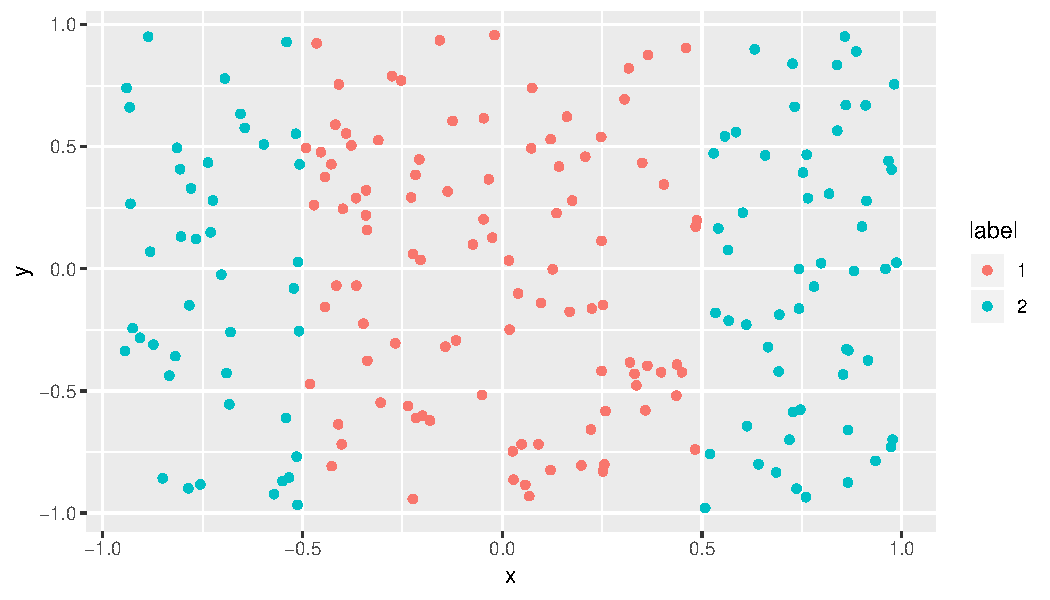
\includegraphics[width=0.85\textwidth]{plots/dat_underlying.pdf}
    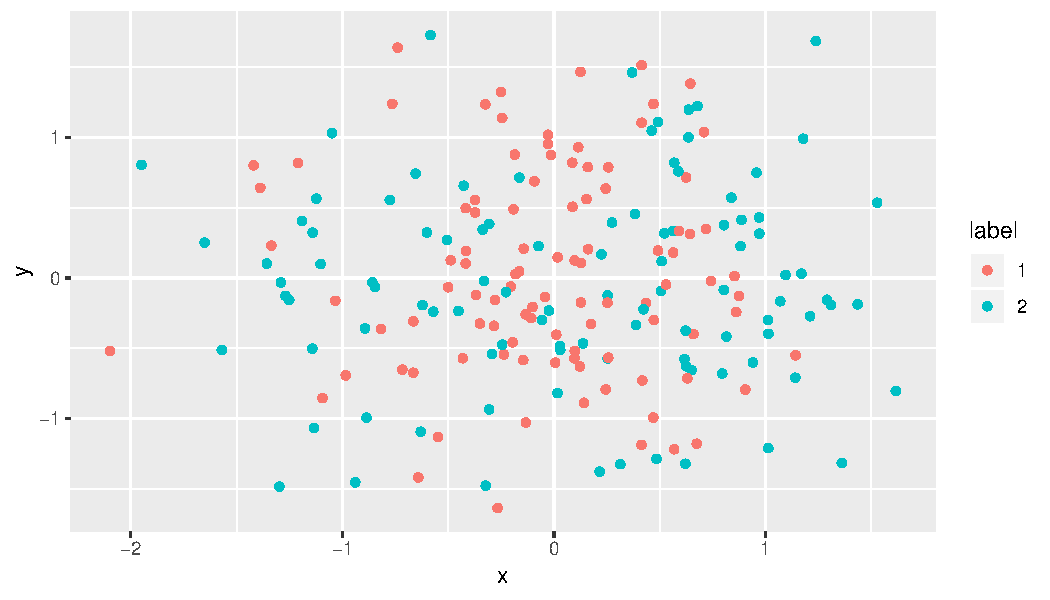
\includegraphics[width=0.85\textwidth]{plots/dat.pdf}
	\caption{Completely observed simulated data: Underlying data generating process (top) and noisy observed data (bottom).}
	\label{fig:simu_data}
\end{figure}

\subsection{Introduction of Missing Values}
For the purpose of this simulation missing values were introduced at random (MAR). The probability of missing observation $X_i$ or $Y_i$ is sampled to be proportional to $X_i$ or $Y_i$, i.e.\
$$P(X_i \text{ missing}) \propto X_i.$$
Observations with






\section{Future Research}
An obvious expansion of this project is to generalize the proposed EM algorithm to Random Forests. Random forests are an ensemble of decorrelated CARTs \citep{breiman} that generally has increased predictive power in comparison with CART.
The EM algorithm for the entire ensemble would simplify to applying the EM algorithm proposed in Section~\ref{EM_for_CART} separately to each of the CARTs in the ensemble. This should result in similar performance improvements.



%%%%%%%%%%%%%%%%%%%%%%%%%%%%%%%%%%%%%%%%%%%%%%%%%%%%%%%%%%%%%%%%%%%%%
\clearpage
\bibliographystyle{dcu} 
{\bibliography{bibliography.bib}}

%%%%%%%%%%%%%%%%%%%%%%%%%%%%%%%%%%%%%%%%%%%%%%%%%%%%%%%%%%%%%%%%%%%%%


\end{document}